

\documentclass[12pt, a4paper]{ article}
\usepackage{graphicx}
\setlength{\topmargin}{0in}
\setlength{\headheight}{0in}
\setlength{\headsep}{0in}
\setlength{\textheight}{9.5in}
\setlength{\textwidth}{6.5in}
\setlength{\oddsidemargin}{0in}
\setlength{\evensidemargin}{0in}


\date{}
\begin{document} 
\title{Blinky Lights} 
\author{Kevin Yeap, Steven Morad, Connie Yu, Reid Anetsberger}
\maketitle 

\noindent
\textbf{1. Hardware:} 

\vspace{1cm}

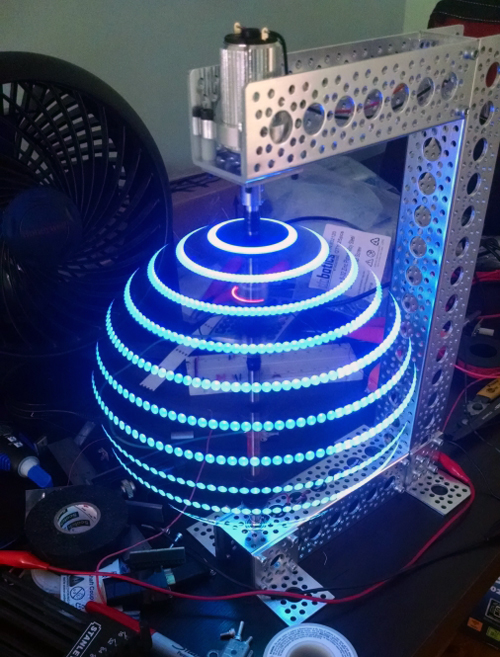
\includegraphics[]{C:/Users/KevinD/Desktop/user_doc/b.PNG}


\vspace {1cm }
1. Plug in the LED orb and turn on the switch to turn on the hardware.

\indent

WARNINGS: hardware spins at high speeds. Do not attempt to touch the hardware when it is spinning. 
Keep out of reach of children under 6 years of age. If you accidentally swallow hardware, seek professional help or contact a poison control center immediately.


\vspace{10cm}





\textbf{2. Bluetooth:} Turn on bluetooth on your pc and sync it to the bluetooth on the hardware. 

\indent


\includegraphics[]{C:/Users/KevinD/Desktop/user_doc/bluetooth.PNG}


\vspace{20cm}
\indent

\textbf{2. Software:} Execute the program . You should be greeted with the following GUI 

\indent

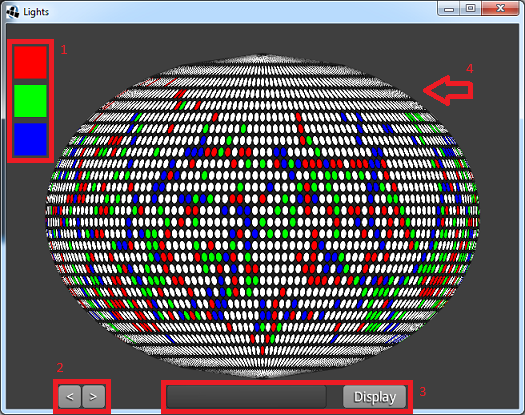
\includegraphics[]{C:/Users/KevinD/Desktop/user_doc/a_labels.PNG}
\vspace{1cm}

1. Click on a color to change the color of your brush
\vspace{1cm}

2. Click on an arrow to change the rotation of the globe.
\vspace{1cm}

3. Type something inside the textbox. Click on the "Display" button to show it on the globe canvas.
\vspace{1cm}

4. A single circle on the globe canvas represents an LED's position  at the time it flashes. Click on it to change its color.





















\end{document}